\documentclass[12pt]{article}
\usepackage[margin=1in]{geometry} 
\usepackage{amsmath}
\usepackage{tcolorbox}
\usepackage{amssymb}
\usepackage{amsthm}
\usepackage{lastpage}
\usepackage{fancyhdr}
\usepackage{accents}
\usepackage{url}
\usepackage[colorlinks]{hyperref}
\usepackage{changepage}
\usepackage{booktabs}
\usepackage[none]{hyphenat}
\usepackage{graphicx}
\usepackage{parskip}
\pagestyle{fancy}
\setlength{\headheight}{40pt}

\newcommand{\indep}{\rotatebox[origin=c]{90}{$\models$}}
\newcommand{\ubar}[1]{\underaccent{\bar}{#1}}

\DeclareMathOperator*{\argmax}{arg\,max}
\DeclareMathOperator*{\argmin}{arg\,min}

\begin{document}

\lhead{Homework \#2 \\ \textbf{Student name: James Hahn} }
\rhead{CS8803 - PGM \\ Probabilistic Graphical Models} 
\cfoot{\thepage\ of \pageref{LastPage}}
\noindent

\textbf{Problem 1}

a) 

Eliminate variables in this order: W, O, M, F, G, B, H

$P(S = true \vert C = true) = \frac{P(S = true, C = true)}{P(C = true)}$

$P(S = true, C = true) = \sum_W\sum_F\sum_O\sum_M\sum_G\sum_B\sum_H P(W)P(O)P(F\vert W, O)P(c)P(M)P(G \vert c, M)\\P(B \vert F, G)P(H \vert s, G)P(s \vert F, B)$

Let $\varphi_W(F, O) = \sum_W P(W)P(F \vert W, O)$

$= \sum_F\sum_O\sum_M\sum_G\sum_B\sum_H P(O)P(c)P(M)P(G \vert c, M)P(B \vert F, G)P(H \vert s, G)P(s \vert F, B)\varphi_W(F, O)$

Let $\varphi_O(F) = \sum_O P(O)\varphi_W(F, O)$

$= \sum_F\sum_M\sum_G\sum_B\sum_H P(c)P(M)P(G \vert c, M)P(B \vert F, G)P(H \vert s, G)P(s \vert F, B)\varphi_O(F)$

Let $\varphi_M(G) = \sum_M P(c)P(M)P(G \vert c, M)$

$= \sum_F\sum_G\sum_B\sum_H P(B \vert F, G)P(H \vert s, G)P(s \vert F, B)\varphi_O(F)\varphi_M(G)$

Let $\varphi_F(B, G) = \sum_F P(B \vert F, G)P(s \vert F, B)\varphi_O(F)$

$= \sum_G\sum_B\sum_H P(H \vert s, G)\varphi_M(G)\varphi_F(B, G)$

Let $\varphi_G(B, H) = \sum_G \varphi_M(G)\varphi_F(B, G)P(H \vert s, G)$

$= \sum_B\sum_H \varphi_G(B, H)$

Let $\varphi_B(H) = \sum_B \varphi_G(B, H)$

$= \sum_H \varphi_B(H)$

$= 0.313192$

So, we have $P(S = true \vert C = true) = \frac{P(S = true, C = true)}{P(C = true)} = \frac{0.313192}{0.4} = \mathbf{0.78298}$

All the factor tables I generated can be seen in the below screenshot. $f_0$ corresponds to the first factor function I created, above, and it follows down such that $f_6 = \varphi_B(H)$. It always shows the final calculation I used to compute the probability above.

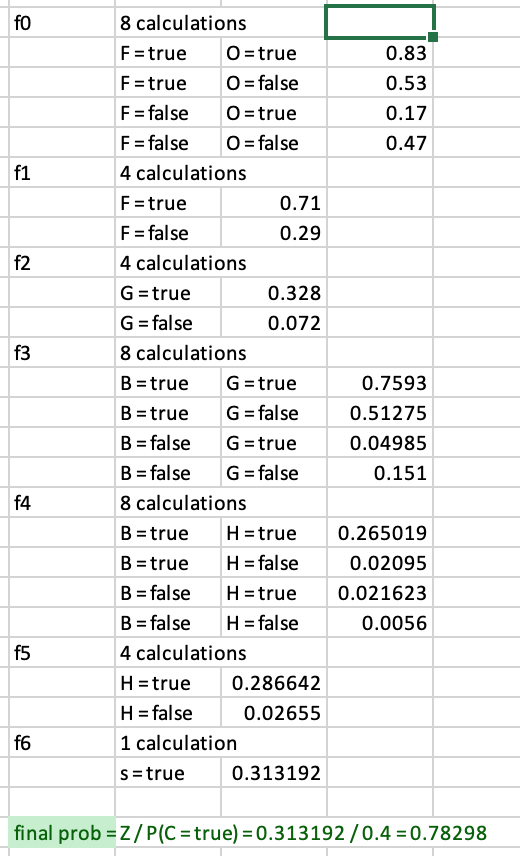
\includegraphics[scale=0.8]{q1-factors}

b) 

$P(F = true \vert G = true) = \frac{P(F = true, G = true)}{\sum_F P(F, G = true)}$

$P(F, G = true) = \sum_W\sum_O\sum_C\sum_M\sum_B\sum_S\sum_H P(W)P(O)P(F\vert W, O)P(C)P(M)P(g \vert C, M)\\P(B \vert F, g)P(H \vert S, g)P(S \vert F, B)$

Let $\varphi_W(F, O) = \sum_W P(W)P(F \vert W, O)$

$= \sum_O\sum_C\sum_M\sum_B\sum_S\sum_H P(O)P(C)P(M)P(g \vert C, M)P(B \vert F, g)P(H \vert S, g)P(S \vert F, B)\varphi_W(F, O)$

Let $\varphi_C(M) = \sum_C P(C)P(g \vert C, M)$

$= \sum_O\sum_M\sum_B\sum_S\sum_H P(O)P(M)P(B \vert F, g)P(H \vert S, g)P(s \vert F, B)\varphi_W(F, O)\varphi_C(M)$

Let $\varphi_M = \sum_M P(M)\varphi_C(M) = 0.7066$

$= 0.7066\sum_O\sum_B\sum_S\sum_H P(O)P(B \vert F, g)P(H \vert S, g)P(s \vert F, B)\varphi_W(F, O)$

Let $\varphi_O(F) = \sum_O P(O)\varphi_W(F, O)$

$= 0.7066\sum_B\sum_S\sum_H P(B \vert F, g)P(H \vert S, g)P(s \vert F, B)\varphi_O(F)$

Let $\varphi_S(F, B, H) = \sum_S P(S\vert F, B)P(H \vert S, g)$

$= 0.7066\sum_B\sum_H P(B \vert F, g)\varphi_O(F)\varphi_S(F, B, H)$

Let $\varphi_H(F, B) = \sum_H \varphi_S(F, B, H)$

$= 0.7066\sum_B P(B \vert F, g)\varphi_O(F)\varphi_H(F, B)$

Let $\varphi_B(F) = \sum_B \varphi_H(F, B)P(B \vert F, G)$

$= 0.7066\varphi_O(F)\varphi_B(F)$

So, $P(F = true, G = true) = 0.71$, $P(F = false, G = true) = 0.29$, and $P(F = true \vert G = true) = \frac{P(F = true, G = true)}{G = true} = \frac{0.71}{0.71 + 0.29} = \mathbf{0.71}$

c) 

$P(M = true \vert G = true) = \frac{P(M = true, G = true)}{\sum_M P(M, G = true)}$

$P(M, G = true) = \sum_S\sum_W\sum_O\sum_C\sum_F\sum_B\sum_H P(W)P(O)P(F\vert W, O)P(C)P(M)P(g \vert C, M)\\P(B \vert F, g)P(H \vert S, g)P(S \vert F, B)$

Let $\varphi_W(F, O) = \sum_W P(W)P(F \vert W, O)$

$= \sum_S\sum_O\sum_C\sum_F\sum_B\sum_H P(O)P(C)P(M)P(g \vert C, M)P(B \vert F, g)P(H \vert S, g)P(S \vert F, B)\varphi_W(F, O)$

Let $\varphi_O(F) = \sum_O P(O)\varphi_W(F, O)$

$= \sum_S\sum_C\sum_F\sum_B\sum_H P(C)P(M)P(g \vert C, M)P(B \vert F, g)P(H \vert S, g)P(S \vert F, B)\varphi_O(F)$

Let $\varphi_B(F, S) = \sum_B P(B \vert F, g)P(S \vert F, B)$

$= \sum_S\sum_C\sum_F\sum_H P(C)P(M)P(g \vert C, M)P(H \vert S, g)\varphi_O(F)\varphi_B(F, S)$

Let $\varphi_H(S) = \sum_H P(H \vert S, g)$

$= \sum_S\sum_C\sum_F P(C)P(M)P(g \vert C, M)\varphi_O(F)\varphi_B(F, S)\varphi_H(S)$

Let $\varphi_C(M) = \sum_C P(C)P(g \vert C, M)$

$= \sum_S\sum_F P(M)\varphi_O(F)\varphi_B(F, S)\varphi_H(S)\varphi_C(M)$

Let $\varphi_F(S) = \sum_F \varphi_O(F)\varphi_B(F, S)$

$= \sum_S P(M)\varphi_H(S)\varphi_C(M)\varphi_F(S)$

Let $\varphi_S = \sum_S \varphi_H(S)\varphi_F(S) = 1$

$= P(M)\varphi_C(M)$

So, $P(M = true, G = true) = 0.0049$, $P(M = false, G = true) = 0.702$, and $P(M = true \vert G = true) = \frac{P(M = true, G = true)}{\sum_M P(M, G = true)} = \frac{0.0049}{0.0049 + 0.702} = \mathbf{0.00651}$

d) 

$P(M = true \vert G = true, S = true) = \frac{P(M = true, G = true, S = true)}{\sum_M P(M, G = true, S = true)}$

$P(M, G = true, S = true) = \sum_W\sum_O\sum_C\sum_F\sum_B\sum_H P(W)P(O)P(F\vert W, O)P(C)P(M)P(g \vert C, M)\\P(B \vert F, g)P(H \vert s, g)P(s \vert F, B)$

Let $\varphi_W(F, O) = \sum_W P(W)P(F \vert W, O)$

$= \sum_O\sum_C\sum_F\sum_B\sum_H P(O)P(C)P(M)P(g \vert C, M)P(B \vert F, g)P(H \vert s, g)P(s \vert F, B)\varphi_W(F, O)$

Let $\varphi_O(F) = \sum_O P(O)\varphi_W(F, O)$

$= \sum_C\sum_F\sum_B\sum_H P(C)P(M)P(g \vert C, M)P(B \vert F, g)P(H \vert s, g)P(s \vert F, B)\varphi_O(F)$

Let $\varphi_B(F) = \sum_B P(B \vert F, g)P(s \vert F, B)$

$= \sum_C\sum_F\sum_H P(C)P(M)P(g \vert C, M)P(H \vert s, g)\varphi_O(F)\varphi_B(F)$

Let $\varphi_H = \sum_H P(H \vert s, g) = 1$

$= \sum_C\sum_F P(C)P(M)P(g \vert C, M)\varphi_O(F)\varphi_B(F)$

Let $\varphi_C(M) = \sum_C P(C)P(g \vert C, M)$

$= \sum_F P(M)\varphi_O(F)\varphi_B(F)\varphi_C(M)$

Let $\varphi_F = \sum_F \varphi_O(F)\varphi_B(F) = 0.80915$

$= 0.80915P(M)\varphi_C(M)$

So, $P(M = true, G = true, S = true) = 0.00372209$, $P(M = false, G = true, S = true) = 0.57174539$, and $P(M = true \vert G = true, S = true) = \frac{P(M = true, G = true, S = true)}{\sum_M P(M, G = true, S = true)} = \frac{0.00372209}{0.00372209 + 0.57174539} = \mathbf{0.006468}$

e) 

$P(W = true \vert G = true, S = true, B = false) = \frac{P(W = true, G = true, S = true, B = false)}{\sum_W P(W, G = true, S = true, B = false)}$

$P(W, G = true, S = true, B = false) = \sum_O\sum_C\sum_F\sum_M\sum_H P(W)P(O)P(F\vert W, O)P(C)P(M)\\P(g \vert C, M)P(b \vert F, g)P(H \vert s, g)P(s \vert F, b)$

Let $\varphi_H(H) = \sum_H P(H \vert s, g) = 1$

$= \sum_O\sum_C\sum_F\sum_M P(W)P(O)P(F\vert W, O)P(C)P(M)P(g \vert C, M)P(b \vert F, g)P(s \vert F, b)$

Let $\varphi_C(M) = \sum_C P(C)P(G \vert C, M)$

$= \sum_O\sum_F\sum_M P(W)P(O)P(F\vert W, O)P(M)P(b \vert F, g)P(s \vert F, b)\varphi_C(M)$

Let $\varphi_M = \sum_M P(M)\varphi_C(M) = 0.7066$

$= 0.7066\sum_O\sum_F P(W)P(O)P(F\vert W, O)P(b \vert F, g)P(s \vert F, b)$

Let $\varphi_O(F, W) = \sum_O P(O)P(F \vert W, O)$

$= 0.7066\sum_F P(W)P(b \vert F, g)P(s \vert F, b)\varphi_O(F, W)$

Let $\varphi_F(W) = \sum_F P(b \vert F, g)P(s \vert F, b)\varphi_O(F, W)$

$= 0.7066P(W)\varphi_F(W)$

So, $P(W = true, G = true, S = true, B = false) = 0.011087$, $P(W = false, G = true, S = true, B = false) = 0.024137$, and $P(W = true \vert G = true, S = true, B = false) = \frac{P(W = true, G = true, S = true, B = false)}{\sum_W P(W, G = true, S = true, B = false)} = \frac{0.011087}{0.011087 + 0.024137} = \mathbf{0.3148}$

\pagebreak\textbf{Problem 2}

See code. Run ``python3 decoder.py'' to run the program. You'll need to install the ``scipy'' and ``xlrd'' packages using pip beforehand since they are used to load matlab files and Excel spreadsheets. The matrix of counts that I found is as follows:

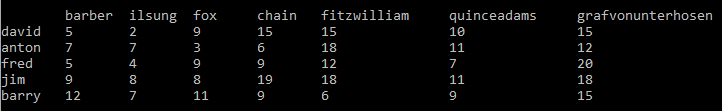
\includegraphics[scale=0.75]{q2-matrix}

It is important to note my 83 state orderings are in order of one hidden state for each firstname, in order of how they appear in the document (david, anton, fred, jim, barry). Each firstname is split into as many states as it has characters, for example david1, david2, david3, david4, david5, representing the characters d, a, v, i, and d respectively. Then, after the firstnames, there are the surnames, with as many hidden states as there are characters in the name, just as I mentioned. Finally, there are 2 intermediate states. Question 2 specifically states there is an initial state that generates random characters until a firstname is chosen, so that is one intermediate state. Then, there is another intermediate state, where we generate random characters again until a surname is chosen. After the surname is finished, the question very explicitly states the model goes back to the beginning of the process, as such it goes back to the initial intermediate state. Since it returns back to the original hidden state, a third intermediate state, following the surname completion, is not required for this HMM. So, there are 22 states for the firstnames, 59 states for the surnames, and 2 intermediate states, totalling 83 states. You can view all the transition and emission probabilities I calculated in the Q2-transitions-and-emissions.xlsx file I provided with this code.

It is important to note there might be slight differences in count matrices between students. In the Viterbi algorithm, when you calculate max, the use of $\geq$ in contrast to just $>$ can cause drastic differences in the final counts matrix. Additionally, the structuring of the states might cause differences in count matrices. I just want to make sure you guys are aware of this while grading this question.

\pagebreak\textbf{Problem 3}

We want to find 

$\argmax_{a, b, c} P(a\vert b)P(b\vert c)P(c) \\
= \argmax_{a}\argmax_{b}\argmax_{c} P(a\vert b)P(b\vert c)P(c) \\
= \argmax_{a}P(a\vert b)\argmax_{b}P(b\vert c)\argmax_{c} P(c)$

Let $\gamma(b) = \sum_c P(b\vert c)P(c)$ and $\gamma(a) = \sum_b P(a \vert b)\gamma(b)$

We get $\gamma(b = true) = 0.36$ and $\gamma(b = false) = 0.64$ with the following table:

\begin{table}[h]
	\begin{tabular}{|l|l|l|}
		\hline
		& b = true & b = false \\ \hline
		c = true  & 0.3      & 0.1       \\ \hline
		c = false & 0.06     & 0.54      \\ \hline
	\end{tabular}
\end{table}

Then, we get $\gamma(a = true) = 0.198$ and $\gamma(a = false) = 0.642$ with the following table:

\begin{table}[h]
	\begin{tabular}{|l|l|l|}
		\hline
		& a = true & a = false \\ \hline
		b = true  & 0.09      & 0.21       \\ \hline
		b = false & 0.108     & 0.432      \\ \hline
	\end{tabular}
\end{table}

As such, we see $\argmax_a \gamma(a)$ leads to \textbf{a = false}. After inspecting the 2nd table above, we see the value of b that contributes the most to $\gamma(a = false)$ is \textbf{b = false}, which is $\argmax_b P(a = true \vert b)\gamma(b)$.

Finally, we want $\argmax_c \gamma(b = false)$. When looking at the first table, the value of c that contributes the most to $\gamma(b = false)$ is when \textbf{c = false}.

So, using the max-product algorithm, through the use of backpointers, we have found argmax of the distribution occurs when \textbf{a = false, b = false, c = false}.

\pagebreak\textbf{Problem 4}

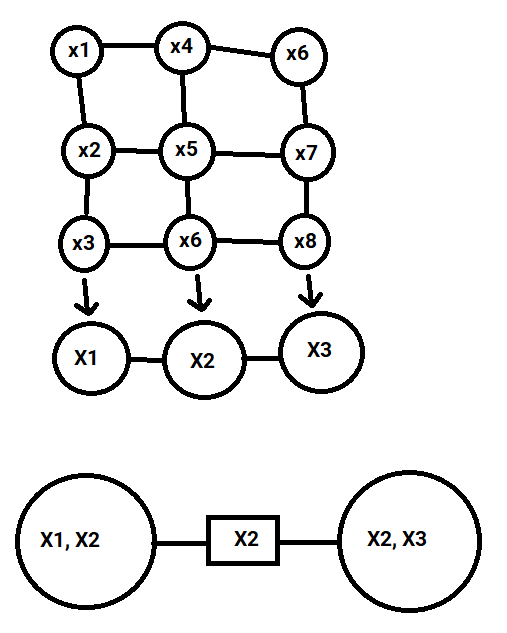
\includegraphics[scale=0.5]{q4}

The generated junction tree is shown in the above diagram where $\phi(X_1, X_2) = \phi(x_1, x_2, x_3, x_4, x_5, x_6)$ and $\phi(X_2, X_3) = \phi(x_4, x_5, x_6, x_7, x_8, x_9)$. Let 

$\phi(X_1, X_2) = \phi(x_1, x_2)\phi(x_2, x_3)\phi(x_1, x_4)\phi(x_2, x_5)\phi(x_3, x_6)\phi(x_4, x_5)\phi(x_5, x_6)$

$\phi(X_2, X_3) = \phi(x_4, x_7)\phi(x_5, x_8)\phi(x_6, x_9)\phi(x_7, x_8)\phi(x_8, x_9)$

$\phi(X_2) = 1$

We can now perform absorptions to calculate Z:

$\phi_1^*(X_2) = \sum_{X_1} \phi(X_1, X_2) = \sum_{x_1, x_2, x_3} = \phi(x_1, x_2)\phi(x_2, x_3)\phi(x_1, x_4)\phi(x_2, x_5)\phi(x_3, x_6)\phi(x_4, x_5)\phi(x_5, x_6)$

$\phi^*(X_2, X_3) = \phi(X_2, X_3)\frac{\phi_1^*(X_2)}{\phi(X_2)} = \phi(X_2, X_3)\phi^*(X_2) = \phi(X_2, X_3)\sum_{X_1} \phi(X_1, X_2)$

$\phi_2^*(X_3) = \sum_{X_2} \phi_1^*(X_2, X_3)$

$\phi^*(X_3, X_4) = \phi(X_3, X_4)\frac{\phi_2^*(X_3)}{\phi(X_3)}$

$\dots$

$\phi_{n-2}^*(X_{n-1}) = \sum_{X_{n-2}} \phi(X_{n-2}, X_{n-1})$

$\phi^*(X_{n-1}, X_n) = \phi(X_{n-1}, X_n)\frac{\phi_{n-2}^*(X_{n-1})}{\phi(X_{n-1})} = \phi(X_{n-1}, X_n)\sum_{X_{n-2}} \phi(X_{n-2}, X_{n-1})\dots \sum_{X_1} \phi(X_1, X_2)$\\

$Z = \sum_{X_{n-1}, X_n} \phi^*(X_{n-1}, X_n) \\
= \sum_{X_{n-1}, X_n} \phi(X_{n-1}, X_n)\sum_{X_{n-2}} \phi(X_{n-2}, X_{n-1}) \dots \sum_{X_2} \phi(X_2, X_3)\sum_{X_1} \phi(X_1, X_2)$

First, we must calculate the big X potentials $\phi(X_i, X_{i+1})$, not to be confused with little x potentials in the original lattice $\phi(x_i, x_{i+1})$. Since each $X_i$ stacks n variables (in an nxn lattice), it takes control of n binary variables. As such, it models $2^n$ possible variable configurations. In the JCT algorithm, since we have $\phi(X_i, X_{i+1})$, we must iterate over $2^n$ states for $X_i$ and $2_n$ states for $X_{i+1}$, for a total of $2^n(2^n) = 2^{2n}$ possible state configurations.

As shown above, for $\phi(X_1, X_2)$, for each state configuration, we must multiply N-1 nodes' vertical edge potentials, which is 2 in our case, then N nodes' horizontal edge potentials, which is N, and finally N-1 node's vertical edge potentials again. This leads to a total of (N-1) + N + (N-1) nodes used for multiplications, or 3N-3 multiplications in total. Then, to generalize this, notice how above $\phi(X_2, X_3)$ has fewer edge potentials than $\phi(X_1, X_2)$. This will be the case for all $\phi(X_i, X_{i+1})$ where $i \neq 1$. In this case, instead of 3n-3 multiplications across 3n-2 nodes, we will instead have 2n-2 multiplications across 2n-1 nodes. As such, to actually generate each pairwise big X edge potential, or in other words initialize them, we require $2^{2n}((3n-3) + (2n-2)) = 2^{2n}(5n-5)$ multiplications.

Now, when we actually want to compute Z, we first want to look at the right-most summation provided above, which is $\sum_{X_1} \phi(X_1, X_2)$. In this case, a new function will be generated such that $\phi_1^*(X_2) = \sum_{X_1} \phi(X_1, X_2)$. For this function, $X_2$ will have $2^n$ states, and the summation will sum across $2^n$ numbers, requiring $2^n - 1$ addition operations. As such, since each state requires $2^n-1$ additions, we get a total of $2^n(2^n-1) = 2^{2n} - 2^n$ operations to compute this function. All functions we will compute after this can be represented as $\phi_i^*(X_{i+1}) = \sum_{X_i} \phi(X_i, X_{i+1})\phi_{i-1}^*(X_i)$. In this case, there are still $2^n - 1$ additions and $2^n$ multiplications for each of the $2^n$ states. As such, to compute these subsequent functions, we require $2^n(2^n + (2^n - 1)) = 2^n(2^{n + 1} - 1) = 2^{2n+1} - 2^n$ calculations. We will have to perform these calculations for n-3 messages, all the way from $\phi_2^*(X_3)$ to $\phi_{n-2}^*(X_{n-1})$. Finally, when we eventually get to the final calculations of Z, we have to compute $\sum_{X_{n-1}, X_n} \phi(X_{n-1}, X_n)\phi_{n-2}^*(X_{n-1})$, which are the left-most values of that summation for Z as shown above. Since there is one multiplication per iteration of the loop, and the loop is iterating over two nodes with $2^n$ states each, there are a total of $2^n(2^n) = 2^{2n}$ loop iterations, leading to $2^{2n}$ multiplications, and it is easy to see there are $2^{2n} - 1$ additions, totaling $2^{2n} + (2^{2n} - 1) = 2^{2n + 1} - 1$ operations. As such, since $\phi_1^*(X_2)$ requires $2^{2n} - 2^n$ operations, $\phi_i^*(X_{i+1})$ requires $2^{2n+1} - 2^n$ for a total of n-3 functions, and $\sum_{X_{n-1}, X_n} \phi(X_{n-1}, X_n)\phi_{n-2}^*(X_{n-1})$ requires $2^{2n + 1} - 1$ operations, we get the following complexity for calculating Z:

$(2^{2n} - 2^n) + (n-3)(2^{2n+1} - 2^n) + (2^{2n+1} - 1)\\
= 2^{2n} - 2^n + n2^{2n+1} - n2^n - 3(2^{2n+1}) + 3(2^n) + 2^{2n+1} - 1\\
= n2^{2n+1} - 3(2^{2n+1}) + 2^{2n+1} + 2^{2n} - 2^n - n2^n + 3(2^n) - 1\\
= 2^{2n+1}(n - 3 + 1) + 2^{2n} - 2^n(1 + n - 3) - 1\\
= 2^{2n+1}(n - 2) + 2^{2n} - 2^n(n - 2) - 1\\
= (n-2)(2^{2n+1} - 2^n) + 2^{2n} - 1\\
= O(n2^{2n})\\
= O(n4^n)$


For n = 10, we have \textbf{log(Z) = 186.7916}.

\pagebreak\textbf{Problem 5}

a) The symptom marginals can be found below:

\begin{table}[h!]
	\begin{tabular}{|l|l|l|l|}
		\hline
		i  & $p(s_i = 1)$ & i & $p(s_i = 1)$ \\ \hline
		1  & 0.4418 & 21 & 0.7613 \\ \hline
		2  & 0.4567 & 22 & 0.6956 \\ \hline
		3  & 0.4414 & 23 & 0.5087 \\ \hline
		4  & 0.4913 & 24 & 0.4200 \\ \hline
		5  & 0.4939 & 25 & 0.3519 \\ \hline
		6  & 0.6575 & 26 & 0.3896 \\ \hline
		7  & 0.5046 & 27 & 0.3260 \\ \hline
		8  & 0.2687 & 28 & 0.4696 \\ \hline
		9  & 0.6491 & 29 & 0.5229 \\ \hline
		10 & 0.4907 & 30 & 0.7173 \\ \hline
		11 & 0.4226 & 31 & 0.5242 \\ \hline
		12 & 0.4291 & 32 & 0.3537 \\ \hline
		13 & 0.5450 & 33 & 0.5127 \\ \hline
		14 & 0.6330 & 34 & 0.5294 \\ \hline
		15 & 0.4295 & 35 & 0.3858 \\ \hline
		16 & 0.4588 & 36 & 0.4891 \\ \hline
		17 & 0.4276 & 37 & 0.6336 \\ \hline
		18 & 0.4043 & 38 & 0.5896 \\ \hline
		19 & 0.5821 & 39 & 0.4232 \\ \hline
		20 & 0.5896 & 40 & 0.5282 \\ \hline
	\end{tabular}
\end{table}

b) Instead of using the JCT algorithm, we can use the following:

$P(s_i) \\
= \sum_{s\backslash s_i}\sum_{d_1\dots d_20} P(s_1, \dots, s_{40}, d_1, \dots, d_{20}) \\
=  \sum_{s\backslash s_i}\sum_{d_1\dots d_20} P(s_1 \vert Pa(s_1))\dots P(s_{40} \vert Pa(s_{40}))\prod_{j = 1}^{20} P(d_j) \\
= \sum_{d_1\dots d_{20}} P(s_i \vert Pa(s_i))\prod_{j = 1}^{20} P(d_j) \\
= \sum_{Pa(s_i)} P(s_i \vert Pa(s_i))P(Pa_1(s_i))P(Pa_2(s_i))P(Pa_3(s_i)) \\$

In the above equations, $s_i$ is the i-th symptom, $d_j$ is the j-th disease, and $Pa_i(s_i)$ is the i-th parent disease of $s_i$. For each $s_i$, there are 3 parent diseases. For example, if the parents of $s_4$ are $d_2, d_8, d_{22}$, then the above probability evaluates to \\$P(s_4) = \sum_{d_2, d_8, d_{22}} P(s_4 \vert d_2, d_8, d_{22})P(d_2)P(d_8)P(d_{22})$.

After implementing this method, it can be seen the max difference between the two sets of probabilities is 3.153e-14.

\pagebreak c) After setting $s_1, \dots, s_5 = 1$ and $s_6, \dots, s_{10} = 2$, we compute the marginals of the diseases as follows:

\begin{table}[h]
	\begin{tabular}{|l|l|l|l|}
		\hline
		j  & $p(d_j = 1)$ & j & $p(d_j = 1)$ \\ \hline
		1  & 0.0298 & 11 & 0.2873 \\ \hline
		2  & 0.3181 & 12 & 0.4898 \\ \hline
		3  & 0.9542 & 13 & 0.8996 \\ \hline
		4  & 0.3966 & 14 & 0.6196 \\ \hline
		5  & 0.4965 & 15 & 0.9205 \\ \hline
		6  & 0.4352 & 16 & 0.7061 \\ \hline
		7  & 0.1875 & 17 & 0.2012 \\ \hline
		8  & 0.7012 & 18 & 0.9085 \\ \hline
		9  & 0.0431 & 19 & 0.8650 \\ \hline
		10 & 0.6103 & 20 & 0.8839 \\ \hline
	\end{tabular}
\end{table}

\pagebreak\textbf{Problem 6}

a) The junction tree can be seen below:

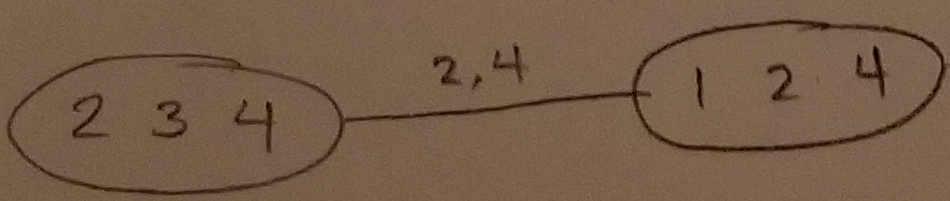
\includegraphics[scale=0.5]{q6-junctiontree-general}

Clearly, this tree has maximal cliques and it is minimal spanning, and it satisfies the running intersection property, so this is the answer to the question.

b) The normal way to calculate the marginal is as follows:

$P(x_1, x_2, x_3, x_4)\\
= \sum_{x_2}\sum_{x_3}\sum_{x_4}\phi(x_1, x_2)\phi(x_2, x_3)\phi(x_3, x_4)\phi(x_4, x_1)\\
= \sum_{x_2}\sum_{x_4}\phi(x_1, x_2)\phi(x_4, x_1)\sum_{x_3}\phi(x_2, x_3)\phi(x_3, x_4)\\
= \sum_{x_2}\sum_{x_4}\phi(x_1, x_2)\phi(x_4, x_1)\phi_{x_3}(x_2, x_4)\\
= \sum_{x_2}\phi(x_1, x_2)\sum_{x_4}\phi(x_4, x_1)\phi_{x_3}(x_2, x_4)\\
= \sum_{x_2}\phi(x_1, x_2)\phi_{x_4}(x_1, x_2)\\
= \phi_{x_2}(x_1)$

Before we go through the whole absorption procedure, this is what the clique tree would roughly look like, along with explicit separators and new nodes that we would calculate in order to retrieve the marginalization of node $x_1$:

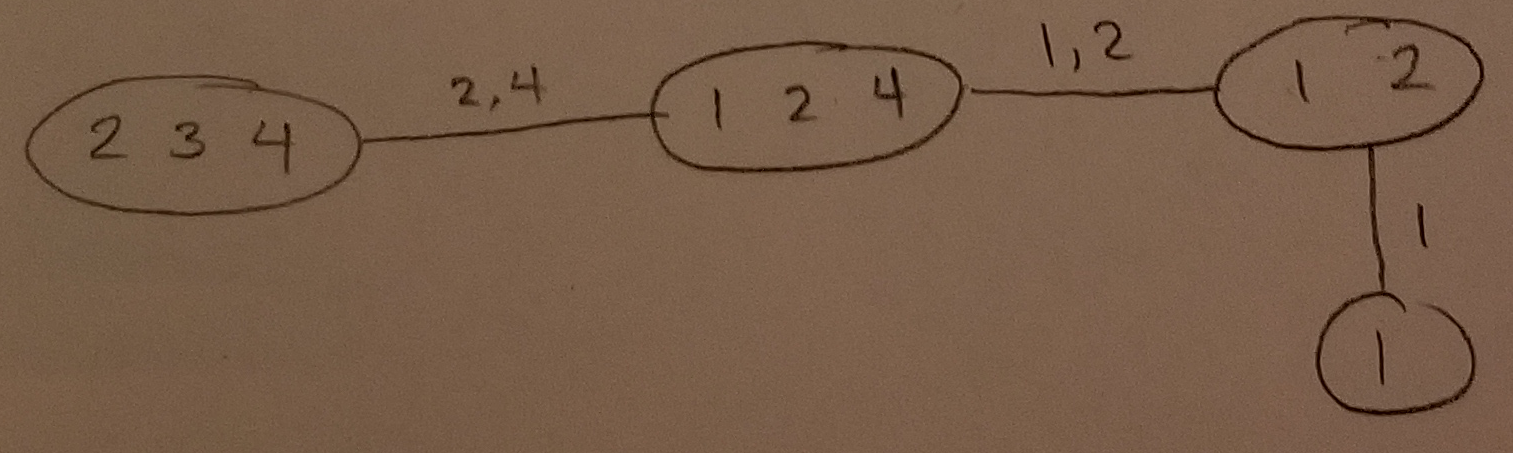
\includegraphics[scale=0.4]{q6-junctiontree}

Now, through the absorption procedure, we get the following:

Let $\phi(x_1, x_2, x_4) = \phi(x_1, x_2)\phi(x_4, x_1)$, $\phi(x_2, x_3, x_4) = \phi(x_2, x_3)\phi(x_3, x_4)$, and $\phi(x_2, x_4) = 1$.

$\phi_1^*(x_2, x_4) = \sum_{x_3}\phi(x_2, x_3, x_4)$

$\phi^*(x_1, x_2, x_4) = \phi(x_1, x_2, x_4)\frac{\phi_1^*(x_2, x_4)}{\phi(x_2, x_4)} = \phi(x_1, x_2, x_4)\frac{\sum_{x_3}\phi(x_2, x_3, x_4)}{\phi(x_2, x_4)} = \phi(x_1, x_2, x_4)\sum_{x_3}\phi(x_2, x_3, x_4)$

$\phi_2^*(x_1, x_2) = \sum_{x_4} \phi^*(x_1, x_2, x_4)$

$\phi^*(x_1, x_2) = \phi(x_1, x_2)\frac{\phi_2^*(x_1, x_2)}{\phi(x_1, x_2)}$

$\phi_3^*(x_1) = \sum_{x_2}\phi^*(x_1, x_2)$

$\phi^*(x_1) = \phi(x_1)\frac{\phi_3^*(x_1)}{\phi(x_1)} = \phi_3^*(x_1)$

As such,w e have computed the marginal of $x_1$, which is $\phi^*(x_1)$. To verify it is the correct result, we will expand the marginal below:

$\phi^*(x_1) \\
= \phi_3^*(x_1) \\
= \sum_{x_2}\phi^*(x_1, x_2) \\
= \sum_{x_2}\phi(x_1, x_2)\frac{\phi_2^*(x_1, x_2)}{\phi(x_1, x_2)} \\
= \sum_{x_2}\frac{\phi(x_1, x_2)}{\phi(x_1, x_2)}\sum_{x_4} \phi^*(x_1, x_2, x_4)\\
= \sum_{x_2}\frac{\phi(x_1, x_2)}{\phi(x_1, x_2)}\sum_{x_4} \phi(x_1, x_2, x_4)\frac{\phi_1^*(x_2, x_4)}{\phi(x_2, x_4)}\\
= \sum_{x_2}\frac{\phi(x_1, x_2)}{\phi(x_1, x_2)}\sum_{x_4} \phi(x_1, x_2, x_4)\frac{\sum_{x_3}\phi(x_2, x_3, x_4)}{\phi(x_2, x_4)}\\
= \sum_{x_2}\sum_{x_3}\sum_{x_4}\frac{\phi(x_1, x_2)}{\phi(x_1, x_2)} \phi(x_1, x_2, x_4)\phi(x_2, x_3, x_4)\frac{1}{\phi(x_2, x_4)}\\
= \sum_{x_2}\sum_{x_3}\sum_{x_4}\frac{\phi(x_1, x_2)}{\phi(x_1, x_2)} \phi(x_1, x_2)\phi(x_4, x_1)\phi(x_2, x_3)\phi(x_3, x_4)\frac{1}{\phi(x_2, x_4)}\\
= \sum_{x_2}\sum_{x_3}\sum_{x_4} \phi(x_1, x_2)\phi(x_4, x_1)\phi(x_2, x_3)\phi(x_3, x_4)\\
= \sum_{x_2}\sum_{x_3}\sum_{x_4} \phi(x_1, x_2)\phi(x_2, x_3)\phi(x_3, x_4)\phi(x_4, x_1)$

This above equation is the exact same equation we got above while we were solving for the marginal of $x_1$ the normal way. As such, we can safely confirm the absorption gives us the correct result.

\pagebreak\textbf{Problem 7}

a) 

The following diagram shows (a) the bayesian network modeling the joint distribution, (b) the bayesian network creating a fully-connected network after moralization, and (c) the junction tree, which is one big node since the network is fully connected:

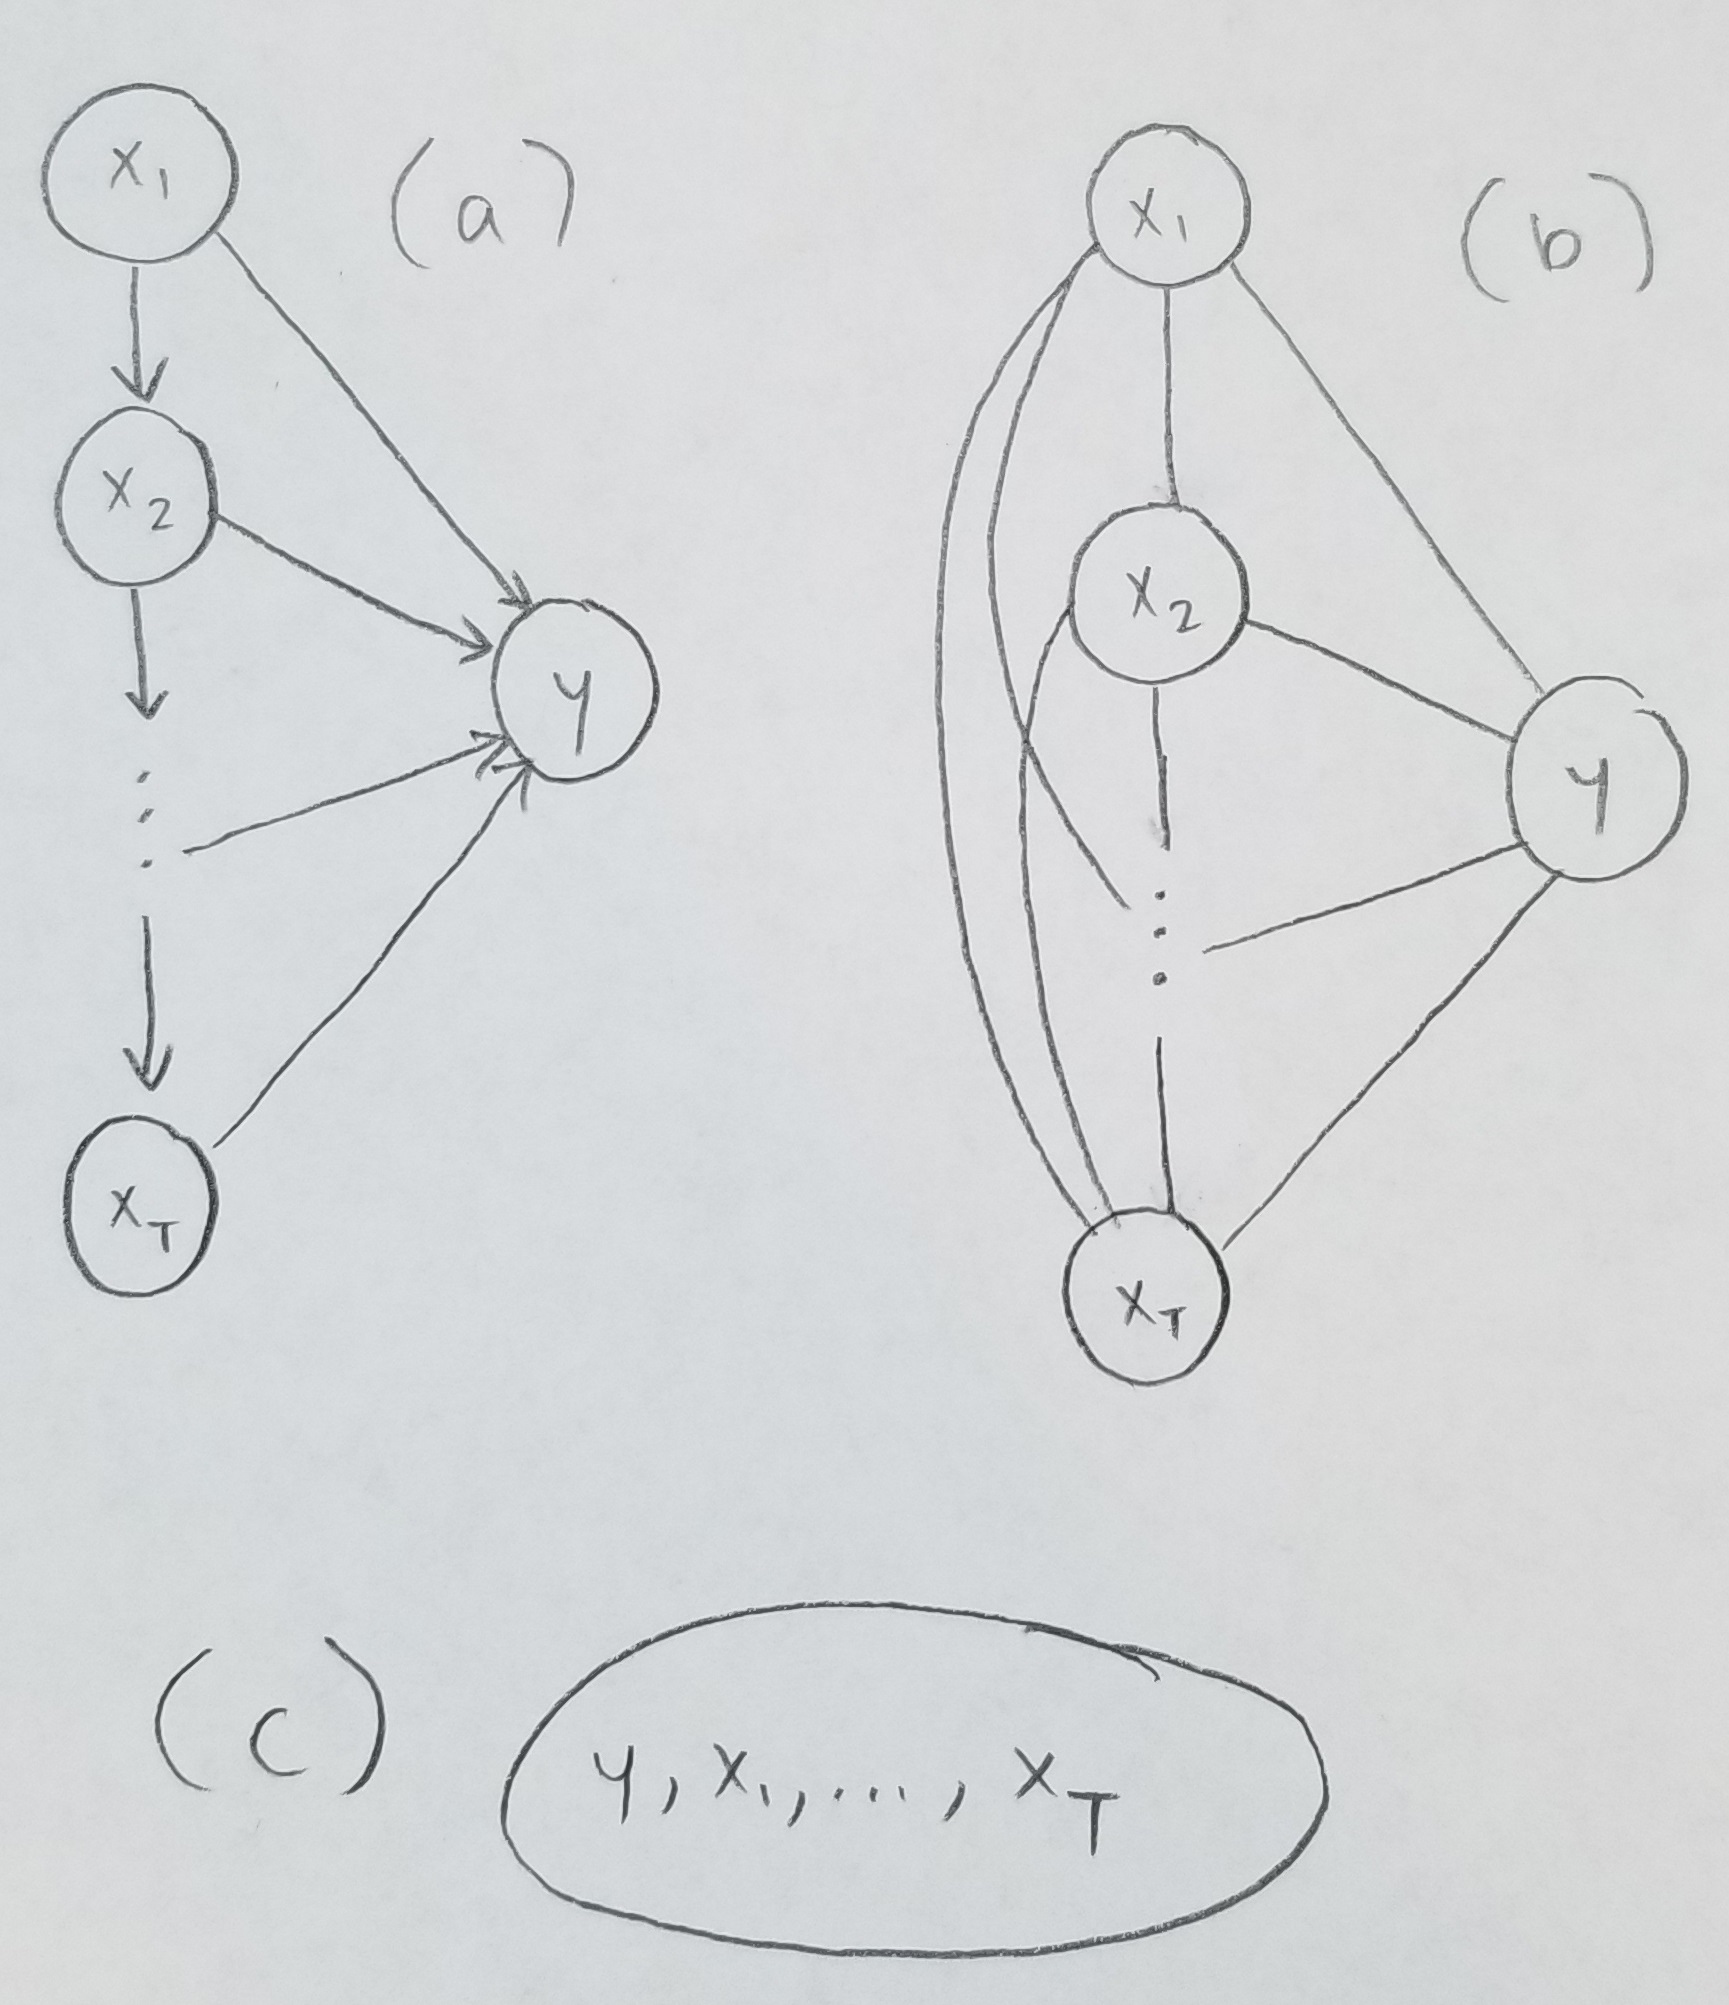
\includegraphics[scale=0.1]{q7-trees}

We want to figure out the runtime complexity of calculating $p(x_T)$ as given by the junction tree algorithm. The junction tree algorithm requires the moralization step. In moralization, two parents of a node must have a direct connection. As such, since all nodes are parents of y, all nodes must be connected to each other, leading to a fully-connected network. Since the network becomes fully-connected after moralization, the junction tree algorithm will give us one huge node containing all nodes in the graph, which is represented as $\phi(y, x_1, \dots, x_T) = p(y \vert x_1, \dots, x_T)p(x_1)\prod_{t = 2}^{T} p(x_t \vert x_{t-1})$. Since all variables are binary, and there are $T+1$ nodes, there are a total of $2^{T+1}$ possible state configurations for this node potential. However, since we want just the potential for $x_T$, we only need to marginalize, or sum, over $T$ nodes, leading to $2^T-1$ additions for each of the two states of $x_T$. Since there are 2 states for $x_T$ and we require $2^T - 1$ additions per state, we require $2(2^T - 1) = 2^{T+1} - 2$ calculations, or $O(2^T)$ time for the junction tree algorithm.

b)

We can reduce this time complexity significantly through variable elimination, as seen below:

$p(x_T) \\
= \sum_{y, x_1, \dots, x_{T-1}} p(y \vert x_1, \dots, x_T)p(x_1)\prod_{t = 2}^{T} p(x_t \vert x_{t-1}) \\
= \sum_{x_1, \dots, x_{T-1}} p(x_1)\prod_{t = 2}^{T} p(x_t \vert x_{t-1}) \sum_y p(y \vert x_1, \dots, x_T)$

We know $\sum_y p(y \vert x_1, \dots, x_T) = 1$.

$= \sum_{x_1, \dots, x_{T-1}} p(x_1)\prod_{t = 2}^{T} p(x_t \vert x_{t-1}) \\
= \sum_{x_1, \dots, x_{T-1}} p(x_1)p(x_2 \vert x_1)\dots p(x_{T-1})p(x_T)$

Let $\varphi_{x_i}(x_{i+1}) = \sum_{x_i} \varphi_{x_{i-1}}(x_i)p(x_{i+1} \vert x_i)$, with a special casing being $\varphi_{x_1} = \sum_{x_1} p(x_1)p(x_{2} \vert x_1)$

$= \sum_{x_2, \dots, x_{T-1}} \varphi_{x_1}(x_2)p(x_3 \vert x_2)\dots p(x_{T-1})p(x_T) \\
= \sum_{x_3, \dots, x_{T-1}} \varphi_{x_2}(x_3)p(x_4 \vert x_3)\dots p(x_{T-1})p(x_T) \\
= \sum_{x_{T-1}} \varphi_{x_{T-2}}(x_{T-1})p(x_T \vert x_{T-1}) \\
= \varphi_{x_{T-1}}(x_{T})$

Each function $\varphi_{x_i}(x_{i+1})$ has two states, and it sums over 2 values, requiring 1 multiplication for each summation. As such, for each state, there are 2 multiplications and 1 addition, totalling $2(2 + 1) = 6$ calculations to compute $\varphi_{x_i}(x_{i+1})$. Since we create $T-1$ of these tables, a total of $6(T-1)$ calculations are required to create all the tables. As such, with this new runtime of $6(T-1) = 6T - 6 = O(T)$, we can see this alternative algorithm is linear in complexity.

\pagebreak\textbf{Problem 8}

a) 

We eliminate the variables in the order $x_{10}$, $x_{9}$, $x_{7}$, $x_{6}$, $x_{5}$, $x_{4}$, $x_{3}$, $x_{2}$, $x_0$ as follows:

$p(x_1 \vert x_{11}, x_8) \\
= \sum_{x_0, x_2, x_3, x_4, x_5, x_6, x_7, x_9, x_{10}} P(0)P(1 \vert 0)P(2 \vert 0)P(3 \vert 0)P(4 \vert 0)P(5 \vert 1, 2, 3, 4)\\P(6 \vert 1, 2, 3, 4)P(7 \vert 1, 2, 3, 4)P(8 \vert 1, 2, 3, 4)P(9 \vert 1, 2, 3, 4)P(10 \vert 1, 2, 3, 4)P(11 \vert 1, 2, 3, 4)$

Note: $x_{11}$ and $x_8$ are given variables, so we do not need to sum over their values. For all other symptoms, they will sum to 1 once they are marginalized out, so we do not need to factor them into the computations.

$= \sum_{x_0, x_2, x_3, x_4} P(0)P(1 \vert 0)P(2 \vert 0)P(3 \vert 0)P(4 \vert 0)P(x_8 \vert 1, 2, 3, 4)P(x_{11} \vert 1, 2, 3, 4)$

Let $\varphi_4(0, 1, 2, 3) = \sum_{x_4} P(4 \vert 0)P(x_8 \vert 1, 2, 3, 4)P(x_{11} \vert 1, 2, 3, 4)$

$= \sum_{x_0, x_2, x_3} P(0)P(1 \vert 0)P(2 \vert 0)P(3 \vert 0)\varphi_4(0, 1, 2, 3)$

Let $\varphi_3(0, 1, 2) = \sum_{x_3} P(3 \vert 0)\varphi_4(0, 1, 2, 3)$

$= \sum_{x_0, x_2} P(0)P(1 \vert 0)P(2 \vert 0)\varphi_3(0, 1, 2)$

Let $\varphi_2(0, 1) = \sum_{x_2} P(2 \vert 0)\varphi_3(0, 1, 2)$

$= \sum_{x_0} P(0)P(1 \vert 0)\varphi_2(0, 1)$

Let $\varphi_0(x_1) = \sum_{x_0} P(0)P(1 \vert 0)\varphi_2(0, 1)$

$= \varphi_0(x_1)$

Now, we will calculate the runtime of this algorithm. For $\varphi_4(0, 1, 2, 3)$, there are 2 multiplications for each iteration, and one addition, resulting in 2(2) + 1 = 5 operations. For $\varphi_3(0, 1, 2)$ requires 1 multiplications for each iteration, and one addition, resulting in 2(1) + 1 = 3 calculations. For $\varphi_2(0, 1)$, there is 1 multiplication per loop iteration, and one addition, resulting in 2(1) + 1 = 3 calculations. Finally, $\varphi_0(1)$ requires 2 multiplications per loop and 1 addition, so 2(2) + 1 = 5 calculations. So, the total number of calculations is 5 + 3 + 3 + 5 = 16 computations.

In terms of space, we need $2^4 = 16$ storage spaces for the entire algorithm since the only factor table we really calculate is $\varphi_4(0, 1, 2, 3)$. When we do individual marginalizations after that, we can do that in place, so we don't need any extra space to compute the additional factor tables.

b) Below is the clique tree:

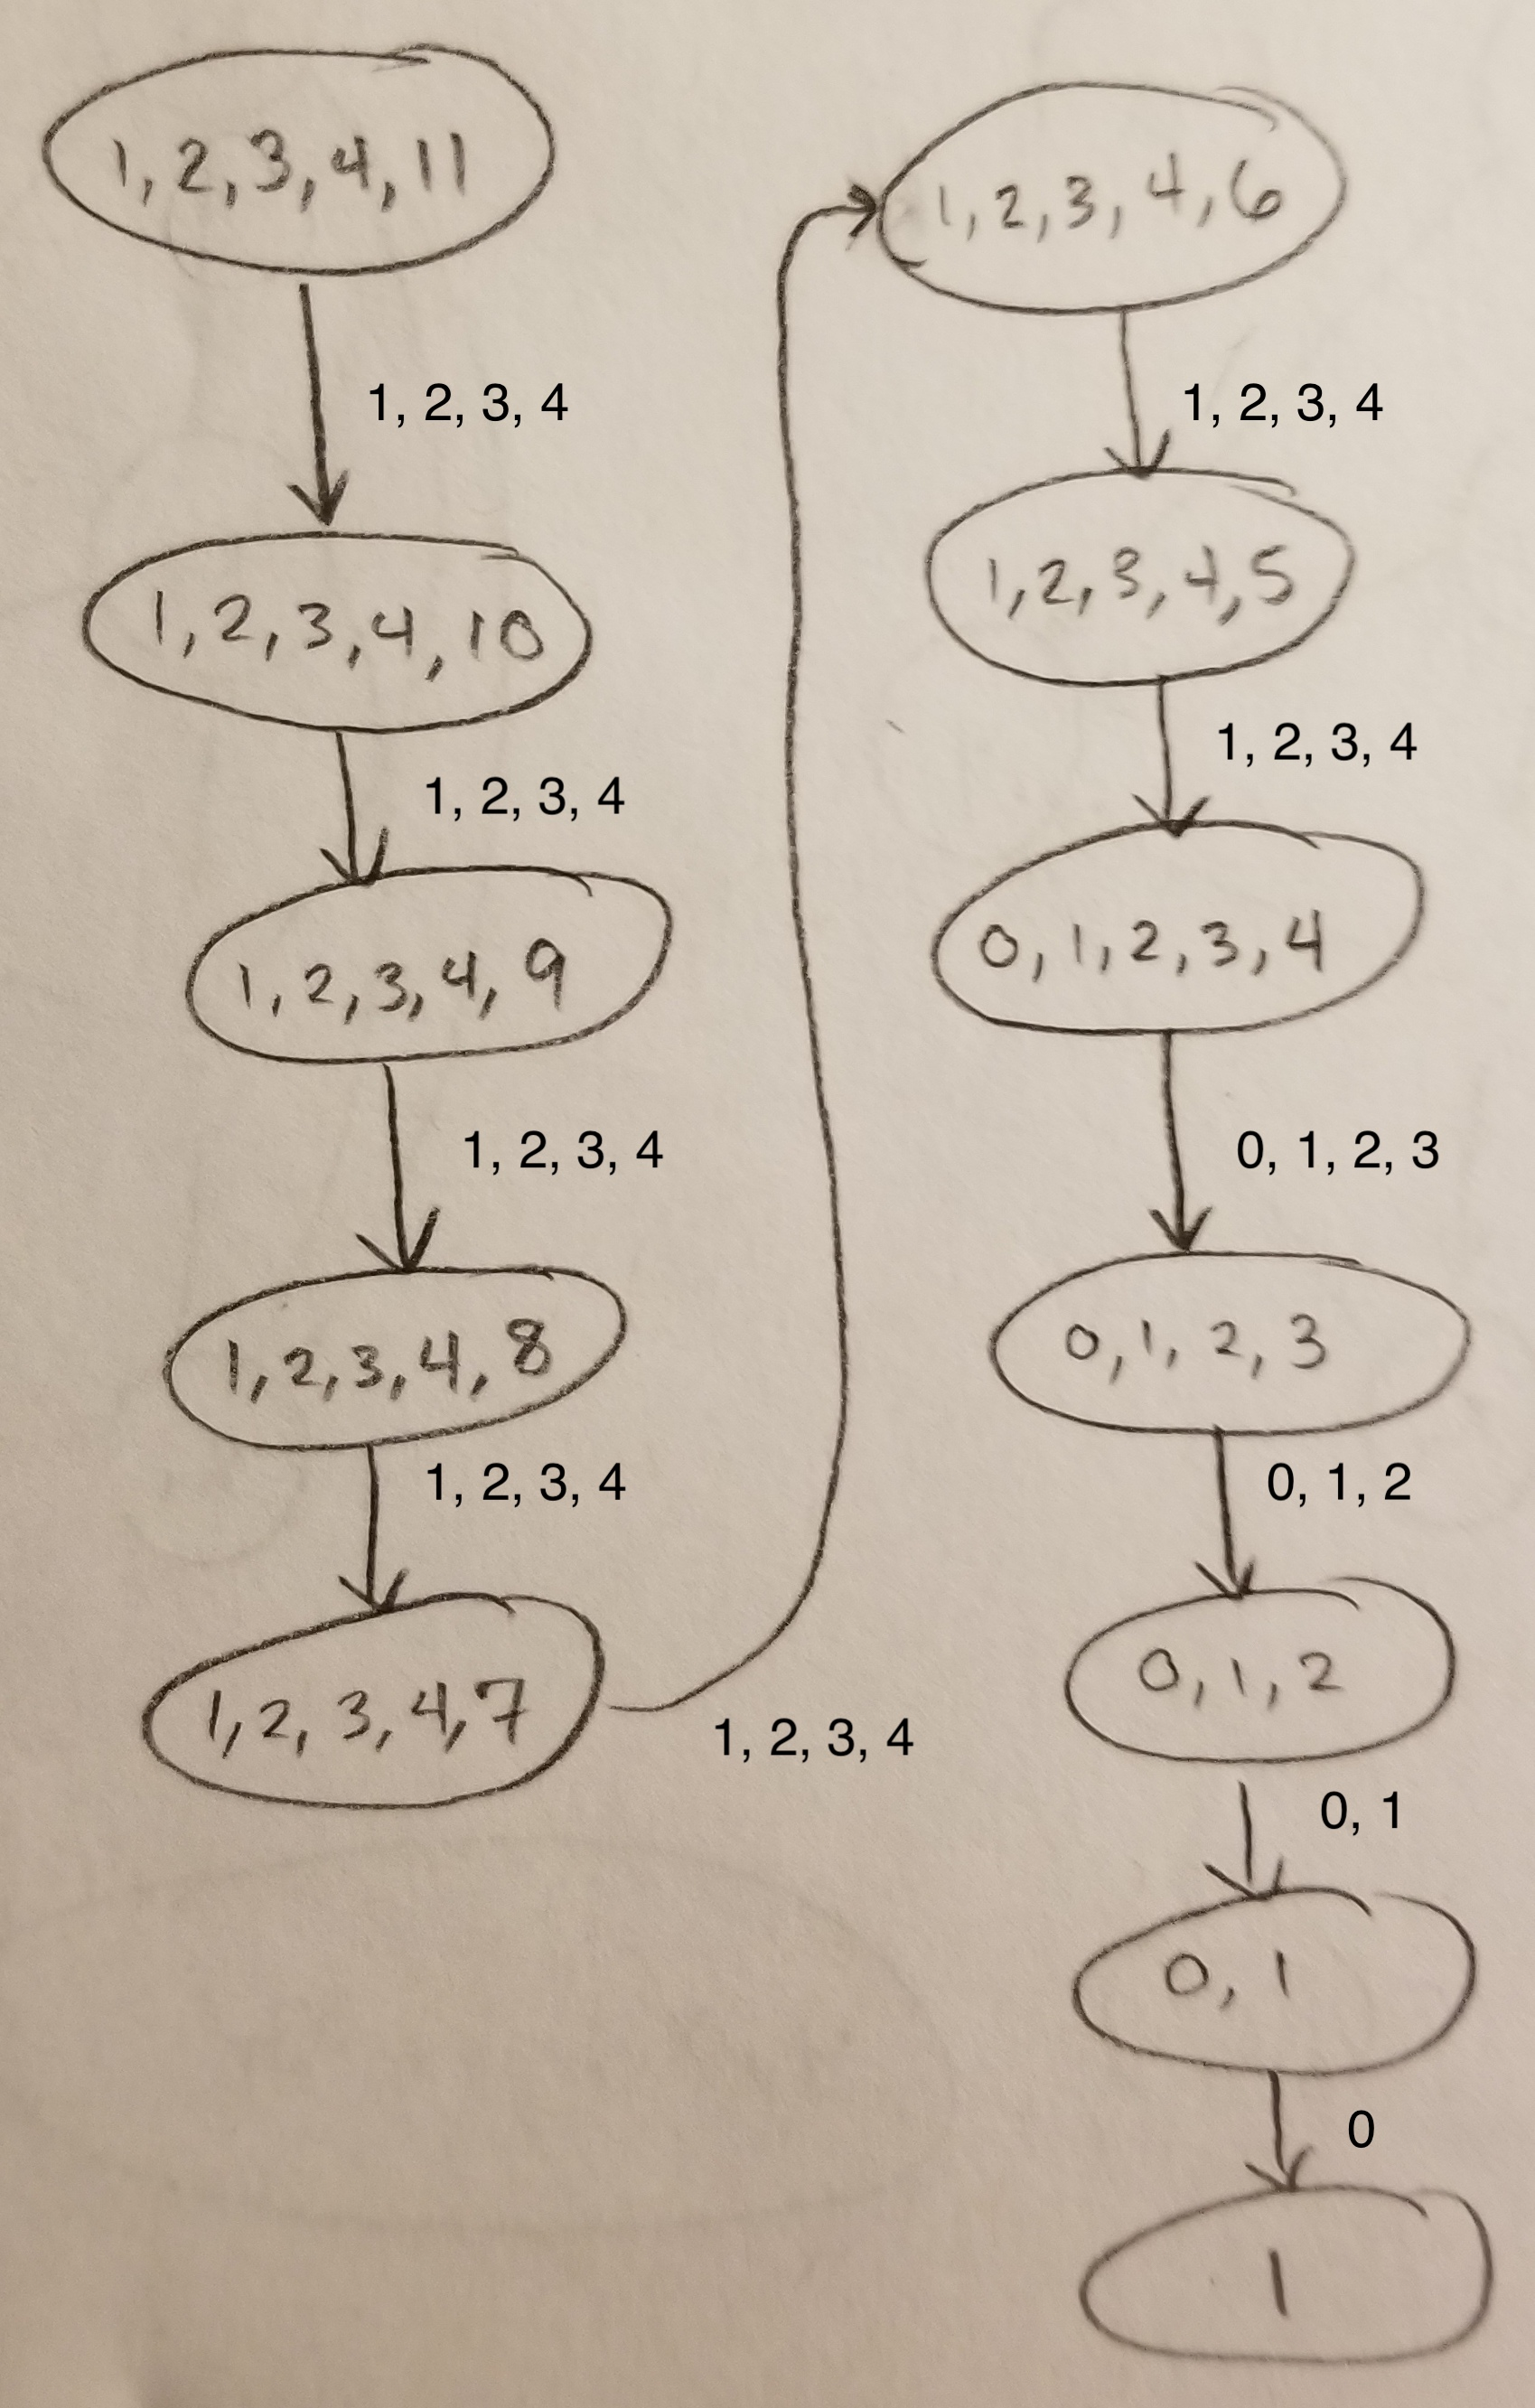
\includegraphics[scale=0.1]{q8b-cliquetree}

(i) The messages here correspond to the distribution of potentials after marginalizing out a given variable. This sub-question is really ambiguous and confusing. Messages are just the result of the tree removing a set of variables. I spoke with Dr. Fekri and he thought it was a little ambiguous as well, or so was inferred from his response. There's nothing special about this junction tree. The first message is just the result of explaining away the 11th node, which is HasFever. This continues, where the next few nodes explain away all the symptoms, then we explain away the diseases, and then finally explain away the IsSummer node. Basically, when a node is not given in a query, that node is kind of removed from the joint distributions, or new factor functions, so we do not have to worry about them again in the future. I'm really just not sure what you're looking for in this question, it's poorly worded, but I think my answer should suffice. In general, the runtime for message passing is O(KN) where K = size of maximal clique. In our case, as seen above, K = 5. So, the runtime is O(5N) = O(N).

As such, the runtime for query 1 would be estimated to be around 5N = 5(11) = 55 operations. As for the space complexity, the biggest tables we have are $2^4 = 16$ + 16 = 32 states because we will need 16 states for the largest node, which is for the node attached to $x_11$ and $x_8$, and then another 16 states for the largest messages that we pass along. So, we need to store both the node states and the messages' states.

(ii) The factors correspond to interactions between diseases and symptoms. For example, some diseases, such as HasFlu, might have a stronger interaction or potential with Coughs, rather than HasRash. As such, the individual factors just compensate for how well the individual symptoms and diseases interact with each other. And then the messages take this information, or these interactions, and pass it onto the next node through message passing.
c) Run ``q8\_c.m'' to get all the tables, which are located in ``symptoms'', ``diseases'', and ``summer\_probs''.

d) The L1 error I am getting is 0.330793. You can run ``q8\_d.m'' to verify. Make sure to run ``q8\_c.m'' beforehand to generate all the tables.

e) I implemented variable elimination. You can test it using ``q8\_e.py''. The necessary libraries you need are scipy. In the below tables a bit being 0 means that variable takes the ``false'' value, and 1 means ``true''.

The result for query 1 is as follows:

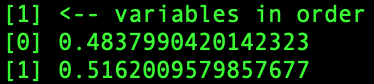
\includegraphics[scale=0.8]{query1}

As we can see, the probability of HasFever = true is 0.5162.

The result for query 2 is as follows:

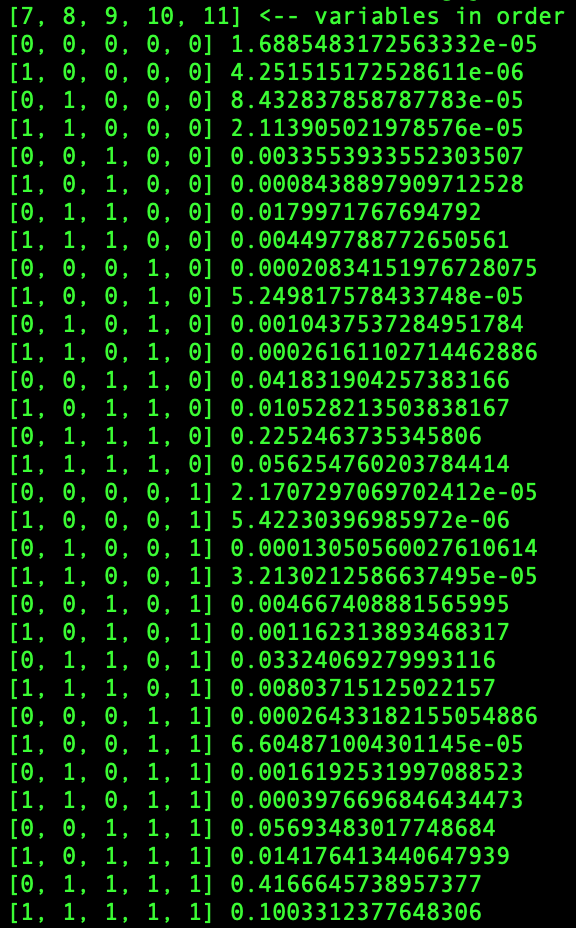
\includegraphics[scale=0.7]{query2}

The above is just simply the probability table for nodes 7, 8, 9, 10, and 11, which is what the question requested. The binary bit values are on the left, and the probability is on the right. I have verified all the probabilities sum to 1, since my program sums up the probabilities to ensure they sum to 1.

The result for query 3 is as follows:

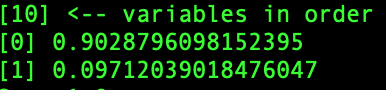
\includegraphics[scale=0.8]{query3}

As seen above, the probability IsSummer = true is 0.0971.

I implemented all the queries in my code. If you want to run my code for a query, you need to modify three lists: ``givens'', ``givenVals'', and ``queries'', which contain the node subscripts for the given nodes (8 and 11 for first query), their given values (1 and 1 for first query -- only other option is 0 for a given node), and finally the node subscripts for the query nodes (1 for first query).

\textbf{Report}

In summary, our model does pretty well. The L1 error from the true distribution is about 0.3308, and considering there are 4096 possible state configurations, that means each parameter is off by 0.3308 / 4096 = 0.000081 on average, which is impressive. We can assume the parameters we estimated are correct. Additionally, we implemented variable elimination suitable for querying this graph, which works well and really shows how efficient our implementation is in practice. I imagine if this graph had like a million nodes the runtime would begin to degrade, but that's much more efficient than the naive implementation of summing over $2^N$ nodes, which might degrade with a thousand nodes.

In terms of the accuracy of the predictions above compared to the true underlying distribution, I am unsure, but I am confident because I computed the 1st and 3rd queries by hand to make sure their probabilities were correct, and they are the same values. However, query 2 was a bit harder since it takes forever to create that table of 32 tables when you have to marginalize over all 4 diseases and the IsSummer node.
\end{document}
